\documentclass[
	preprint,%twocolumn
	aps,
	prb,
	showpacs,	
	amsmath, amssymb]{revtex4-2}
%---packages----------------------------------------------------------
%\usepackage[top=1.25in, bottom=1.25in, left=1.25in, right=1.25in]{geometry}
\usepackage{bm}
\usepackage{graphicx}
\usepackage{hyperref}% add hypertext capabilities
\hypersetup{colorlinks=true, 
			citecolor=blue, 
			urlcolor=blue, 
			linkcolor=blue}
\pdfstringdefDisableCommands{\let\bm=\relax}
\usepackage{scalerel}
\usepackage{cleveref}
\usepackage{tikz} % flow chart
\usetikzlibrary{positioning, shapes.geometric}


%--setups--------------------------------------------------------------
\DeclareRobustCommand{\xjoinrel}{\mathrel{\mkern-4mu}}
\DeclareRobustCommand{\gong}{\hstretch{1.25} {\boldsymbol{\mathrel{|} \xjoinrel\mathrel{-} \xjoinrel\mathrel{|}}}}
%\DeclareRobustCommand{\gong}{\hstretch{1.25} {\boldsymbol{\vdash \xjoinrel\dashv }}}
%\DeclareRobustCommand{\wang}{\hstretch{1.25} {\boldsymbol{\vdash \xjoinrel \mathrel{+} \xjoinrel\dashv }}}
\DeclareRobustCommand{\wang}{\hstretch{1.25} {\boldsymbol{\mathrel{|}  \xjoinrel\mathrel{-} \xjoinrel\mathrel{|} \xjoinrel\mathrel{-} \xjoinrel\mathrel{|}}}}
\DeclareRobustCommand{\+}{\hstretch{1.25} {\boldsymbol {\mathrel{+}}}}
\DeclareRobustCommand{\manyplus}{\hstretch{1.25} {\boldsymbol{ \mathrel{+}\xjoinrel \mathrel{+}\xjoinrel\mathrel{+} \xjoinrel\mathrel{+}}  }}
\DeclareRobustCommand{\l}{\hstretch{1.25} {\boldsymbol {\vdash }}}
\DeclareRobustCommand{\r}{\hstretch{1.25} {\boldsymbol {\dashv }}}
%\DeclareRobustCommand{\tu}{\hstretch{1.25} {\boldsymbol {\mathrel{+} \xjoinrel\dashv }}}
\DeclareRobustCommand{\tu}{\hstretch{1.25} {\boldsymbol{\mathrel{-} \xjoinrel\mathrel{|} \xjoinrel\mathrel{-} \xjoinrel\mathrel{|}}}}
%\DeclareRobustCommand{\tl}{\hstretch{1.25} {\boldsymbol {\xjoinrel\dashv \mathrel{+}}}}
\DeclareRobustCommand{\tl}{\hstretch{1.25} {\boldsymbol{\mathrel{|}  \xjoinrel\mathrel{-} \xjoinrel\mathrel{|} \xjoinrel\mathrel{-} }}}

\newcommand{\tr}{ {\rm Tr} }
\newcommand{\I}{ {\mathbb I} }
\newcommand{\im}{ {\mathrm{Im}} }
\newcommand{\sgn}{ {\mathrm{Sgn}} }

%=======================================================================
%=======================================================================
\begin{document}
\title{Notes: Nevanlinna analytical Continuation Method}
\author{Shuang Liang}
\email{sliang@iphy.ac.cn}
\affiliation{Institute of Physics, Chinese Academy of Sciences}


%\author{Shuang Liang}
%\affiliation{Institute of Physics, Chinese Academy of Sciences}
%\email{sliang@iphy.ac.cn}

\date{\today}
\begin{abstract}
	This is the abstract.
\end{abstract}


\maketitle
\tableofcontents

\newpage
%=====================================================================
%=====================================================================
\section{The analytic continuation problem}
\label{sec:the-analytic-continuation-problem}

The analytic continuation problem seeks   
to extract real frequency dynamical information from
imaginary-time correlation functions $G(\tau)$ data.
Technically, this is a highly nontirvial task\cite{jarrell1996bayesian}. To 
see this, we use the relation between $G(\tau)$ and $A(\omega)$
\cite{jarrell1996bayesian,XiaoLRT}:
\begin{equation}\label{eq:gt-Aw}
	G(\tau) = \int_{-\infty}^{\infty} d\omega
		\frac{e^{-\tau \omega }}{1 - \lambda e^{-\beta \omega}}
		A(\omega)
		= \int_{-\infty}^{\infty} d\omega
		K(\tau, \omega) A(\omega)
\end{equation}
where $K(\tau, \omega) = \frac{e^{-\tau \omega }}{1 - \lambda e^{-\beta \omega}}$
is the kernel. One may consider to solve the problem by firstly 
discretize $\tau$ and $\omega$ and get:
\begin{equation}
	G(\tau_i) = \sum_{j=1}^{N_\omega} K_{ij} A(\omega_j)
\end{equation}
Then do SVD decomposition of rectangular matrix $K$, write
$K_ij = U_{il} \lambda_l V_{lj}$. Finally the spectral function 
reads
\begin{equation}
	A(\omega_j) = \sum_{l=1}^{N_\tau} \frac{1}{\lambda_l} V_{ij}
		\sum_{i=1}^{N_\omega} G(\tau_i) U_{il}
\end{equation}
It seems fine at the first glanse. However, if we consider 
the properties of $K(\tau, \omega)$, we would notice that it 
is highly sigular since it is exponentially small for large 
$|\omega|$, so small errors $G(\tau)$ would be amplified by
exponentially small $\lambda_l$. This problem is well-known
ill-posed\cite{acton1997numerical, peschel1999density} and 
enormous efforts have been made\cite{}.


%=====================================================================
%=====================================================================
\section{How to solve?}
\label{sec:how-to-solve}

$\cdots$

Here we introduce the recently developed Nevanlinna 
analytic continuation method\cite{fei2021nevanlinna}.      
%=====================================================================
%=====================================================================
\section{Nevanlinna analytic continuation}
\label{sec:nevanlinna-analytical-continuation}


%=====================================================================
\subsection{Schur algorithm}
\label{subsec:schur-algorithm}


The Nevanlinna analytic continuation method\cite{fei2021nevanlinna} 
is basically an interpolation method. In this method, one should firstly using 
conformal transforms to map the Masubara Green's functions $\mathcal{G}$, 
which is analytic in the upper half of the complex plane $\mathcal{C}^+$ and 
contains singularities in the lower half plane, to a closed unit disk 
$\bar{\mathcal{D}}$ in the complex plane. The mappings are shown in \cref{fig:conformal-map}. 
It becomes a Schur class($\mathcal{S}$) 
function and would have a continued fraction expansion where the parameters 
can be rescrsively defined\cite{schur1918potenzreihen}. Then one can 
apply the Nevanlinna iterative algorithm to interpolate the Schur 
functions\cite{nevanlinna1919uber}.
Finally, one can do a inverse conformal transform back to $\mathcal{C}^+$ and 
obtains $\mathcal{G}(z)$, it's then natural to do analytic continuation 
$z \to \omega + i0^+$. The calculation process is shown in \cref{fig:calculation-flow-chart}.

\begin{figure}[htbp]
	\centering
	\begin{minipage}[t]{0.7\linewidth}
		\centering
		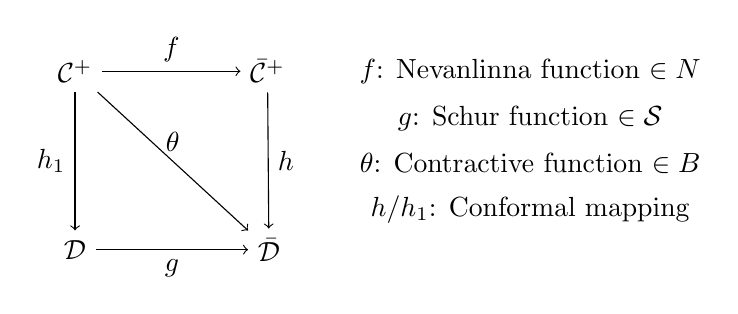
\begin{tikzpicture}[node distance=50pt]
			\node[draw=none,fill=none]  (C)  {$\mathcal{C}^+$};
			\node[draw=none,fill=none, right=of C]  (Cbar)  {$\bar{\mathcal{C}}^+$};                 
			\node[draw=none,fill=none, below=of C]  (D)     {$\mathcal{D}$};               
			\node[draw=none,fill=none,right=55pt of D]  (Dbar)  {$\bar{\mathcal{D}}$};
		
			\draw[->] (C)  -- node[above] {$f$} (Cbar) ;
			\draw[->] (C)  -- node[left] {$h_1$} (D) ;
			\draw[->] (C)  -- node[above] {$\theta$} (Dbar) ;
			\draw[->] (Cbar) -- node[right] {$h$} (Dbar) ;
			\draw[->] (D) -- node[below] {$g$} (Dbar) ;

			\node[draw=none,fill=none, right=20pt of Cbar] (f) {$f$: Nevanlinna function $\in N$};
			\node[draw=none,fill=none, below=1pt of f]  (g)  {$g$: Schur function $\in \mathcal{S}$};                 
			\node[draw=none,fill=none, below=1pt of g]  (t)     {$\theta$: Contractive function $\in B$};               
			\node[draw=none,fill=none,below=1pt of t]  (h)  {$h/h_1$: Conformal mapping};
		\end{tikzpicture}
	\end{minipage}
	\caption{Conformal mappings}
	\label{fig:conformal-map}
\end{figure}

\begin{figure}[htbp]
	\centering
	\begin{minipage}[t]{0.9\linewidth}
		\centering
		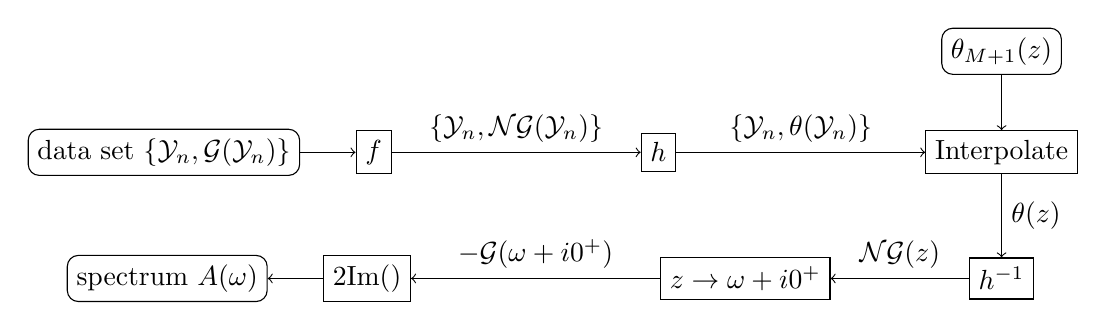
\begin{tikzpicture}[node distance=90pt]
			\node[draw,rounded corners]  (start)  {data set $\{\mathcal{Y}_n, \mathcal{G}(\mathcal{Y}_n)\}$};
			\node[draw,right=20pt of start]  (f)  {$f$};                 
			\node[draw, right=of f]  (h)     {$h$};               
			\node[draw,right=of h]  (interpolate)  {Interpolate};
			\node[draw,rounded corners,above=20pt of interpolate]  (tm)  {$\theta_{M+1}(z)$};
			\node[draw, below=30pt of interpolate]  (invh)  {$h^{-1}$};
			\node[draw, left=50pt of invh]  (ac)  {$z \to \omega + i0^+$};
			\node[draw, left=of ac]  (imag)  {$2\im()$};
			\node[draw, rounded corners, left=20pt of imag]  (end)  {spectrum $A(\omega)$};

			\draw[->] (start) -- (f) ;
			\draw[->] (f)  -- node[above] {$\{\mathcal{Y}_n, \mathcal{NG}(\mathcal{Y}_n)\}$} (h) ;
			\draw[->] (h)  -- node[above] {$\{\mathcal{Y}_n, \theta(\mathcal{Y}_n)\}$} (interpolate) ;
			\draw[->] (tm) -- (interpolate) ;
			\draw[->] (interpolate) -- node[right] {$\theta(z)$} (invh) ;
			\draw[->] (invh) -- node[above] {$\mathcal{NG}(z)$} (ac) ;
			\draw[->] (ac) -- node[above] {$-\mathcal{G}(\omega + i0^+)$} (imag) ;
			\draw[->] (imag) -- (end) ;
		\end{tikzpicture}
	\end{minipage}
	\caption{Calculation flow chart}
	\label{fig:calculation-flow-chart}
\end{figure}

For fermionic Green's functions, the mapping from $\mathcal{C}^+$ to 
$\bar{\mathcal{C}^+}$ is simple. Since $\im \mathcal{G}(z) \leq 0$ if 
$z \in \mathcal{C}^+$, the mapping is just to take 
$\mathcal{G} \to -\mathcal{G} = \mathcal{NG}$ and $\mathcal{NG} \subset N$. While for 
bosonic Green's functions, this mapping is a little bit complicated and 
we will discuss in the next section. The data set we have is 
$\{i\omega_n, \mathcal{G}(i\omega_n)\}$, here we denote $\mathcal{Y}_n = i\omega_n$ 
and $\mathcal{C}_n = \mathcal{NG}(i\omega_n) = -\mathcal{G}(i\omega_n)$. 

Then we use the Möbius transform
\begin{equation}\label{eq:Mobius-transform}
	h(z) = \frac{z - i}{z + i}
\end{equation}
to map $\mathcal{C}_n \subset N$ to 
$\theta(\mathcal{Y}_n) = h(\mathcal{C}_n) \subset \bar{\mathcal{D}}$. 
The recursive final $\theta(z)$ can conveniently be written in a
matrix form:
\begin{equation}\label{eq:recursive-theta}
	\theta(z)[z;\theta_{M+1}(z)] 
		= \frac{a(z)\theta_{M+1}(z) + b(z)}{c(z)\theta_{M+1}(z) + d(z)}
\end{equation}
where
\begin{equation}\label{eq:factor-matrix}
	\left(
		\begin{matrix}
			a(z) & b(z) \\
			c(z) & d(z)
		\end{matrix}
	\right) = \prod_{n=1}^M
	\left(
		\begin{matrix}
			h_1(z, \mathcal{Y}_j) & \phi_j \\
			\phi_j^* h_1(z, \mathcal{Y}_j) & 1
		\end{matrix}
	\right)
\end{equation}
where $h_1(z, \mathcal{Y}_n) = \frac{z - \mathcal{Y}_n}{z -\mathcal{Y}_n^*}$ 
is a conformal map form $\mathcal{C}^+$ to $\mathcal{D}$. $\theta_j(z)$ is 
the interpolation function of $j$-th step and
$\phi_j = \theta_j(\mathcal{Y}_j)$. There is a freedom to choose $\theta_{M+1}(z)$.
One can use this freedom to select the “best” of all consistent spectral functions.

%=====================================================================





\bibliographystyle{unsrt} %引用顺序
\bibliography{nevanlinna.bib}
\end{document}